\chapter{The Proposed Centralized Solution}\label{cha:existingSystem}

The \ref{PS:Q:Scalability} question in the problem statement(\cref{sec:problemStatement}) asks for a comparison between the decentralized solution and the current system at Siemens on different parameters. Ideally, for us to compare the two systems on equal terms, both systems should be implemented in the same environment. However, since we do not have access to the environment where the current system at Siemens is implemented, we have chosen to build our own version of the current Siemens system, in the same environment as the decentralized solution.

This version of the current Siemens system, from now on referred to as the centralized solution, is built from what Siemens has informed about the current Siemens system. The goal of the centralized solution is to create a foundation for a comparison between the decentralized solution and the current Siemens system, by making the system architecture around the regulation algorithm the only parameter changed from the centralized solution to the decentralized solution, thus ruling out the environment difference of the two systems as a parameter. This means the centralized solution is only built to enable us to collect data that can be used to compare the two systems. As a result, we aim to compare the decentralized solutions test results with the centralized solutions test results, collected within the same environment, to more accurately answer the \cref{PS:Q:Scalability} question.

However in order to completely answer the \ref{PS:Q:Scalability} question, and compare the decentralized solution with the current Siemens system, another comparison must be introduced: A comparison between our centralized solution and the current Siemens system. This comparison is relevant in order to close the remaining 'comparison-gap' between the decentralized solution and the current Siemens system. This comparison will be a theoretical comparison between the centralized solution and the current Siemens system, and based on assumptions made when building the centralized solution.

The thesis motivation (\cref{sec:ThesisMotivation}) describes a brief overview of the current system at Siemens. This chapter gives a detailed description of the key component of the current Siemens system: The regulation algorithm. Furthermore the chapter describes the centralized solution followed by a theoretical comparison between the centralized solution and the current Siemens system. 

\section{Regulation algorithm}\label{sec:regAlgorithm}

The regulation algorithm is a key component of the system and it is where new setpoints are calculated. Since the purpose of this thesis is not to improve any regulation algorithms, the regulation algorithm has been considered a black box in development of both the centralized and the decentralized solution. What is important to this thesis is that the algorithm used is the same in both the centralized and the decentralized solution, to make sure the two systems are compared on the same terms. 

To get as realistic a picture of the system as possible of the regulation algorithm, we tried to gain access to the algorithm Siemens currently use, but due to the regulation algorithm at Siemens being a commercial secret, this was not possible.

\begin{figure}
	\centering
	\begin{tikzpicture}[
	point/.style={inner sep=0pt}, %circle,minimum size=2pt,fill=red},
	textNode/.style={inner sep=2pt},
	hv path/.style={to path={-| (\tikztotarget)}},
	vh path/.style={to path={|- (\tikztotarget)}},
	skip loop h/.style={to path={-- ++(0,#1) -| (\tikztotarget)}},
	skip loop v/.style={to path={-- ++(#1,0) |- (\tikztotarget)}},
	graphs/every graph/.style={edges=rounded corners}
	]
	
% Place nodes
\matrix[row sep=1.4cm,column sep=.4cm] {
	\node [point]  		(p1x1)	{}; &&
	\node [rectangle]	(Turbine)		[draw, label=above:\textbf{$\cdot$}N Turbines, text width=50pt]	{Cur.Prod. Max.Prod}; &&
	\node [point]  		(p1x3)	{}; \\
	
	\node [point]  		(p2x1)			{}; &&
	\node [textNode]	(HPPP)		 	{Reg. algorithm}; &&
	\node [textNode]	(Setpoint)	{N Setpoints}; \\

	&& \node [textNode]  (gSetpoint)							{Global SetPoint}; \\
};
	
\graph[use existing nodes]{
	Turbine ->[skip loop v=-3.1cm] HPPP -> Setpoint ->[vh path] Turbine;
	gSetpoint -> HPPP;
};

\end{tikzpicture}



%\begin{tikzpicture}[
%	point/.style={inner sep=0pt}, %circle,minimum size=2pt,fill=red},
%	textNode/.style={inner sep=2pt},
%	hv path/.style={to path={-| (\tikztotarget)}},
%	vh path/.style={to path={|- (\tikztotarget)}},
%	skip loop h/.style={to path={-- ++(0,#1) -| (\tikztotarget)}},
%	skip loop v/.style={to path={-- ++(#1,0) |- (\tikztotarget)}},
%	graphs/every graph/.style={edges=rounded corners}
%	]
%	
%% Place nodes
%\matrix[row sep=1.5cm,column sep=.5cm] {
%	\node [point]  		(p1x1)	{}; &&
%	\node [rectangle]	(Turbine)		[draw, label=above:\textbf{$\cdot$}N Turbines, text width=50pt]	{Cur.Prod. Max.Prod}; &&
%	\node [point]  		(p1x3)	{}; \\
%	
%	\node [point]  		(p2x1)			{}; &&
%	\node [textNode]	(HPPP)		 	{HPPP}; &&
%	\node [textNode]	(Setpoint)	{\textbf{$\cdot$}N Setpoints}; \\
%
%	\node [textNode]  (gSetpoint)										{Global SetPoint}; &&
%	\node [rectangle]	(Data)			[draw, text width=50pt] {Cur.prod  Max.Prod};\\
%};
%
%\node [textNode,right of=Data] {~~~~~~~~~~~~~~~~~\textbf{$\cdot$}N Turbines};
%	
%\graph[use existing nodes]{
%	Turbine ->[skip loop v=-2.7cm] HPPP -> Setpoint ->[vh path] Turbine;
%	gSetpoint.east -> HPPP;
%	Data -> HPPP;
%};
%
%\end{tikzpicture}

	\captionsetup{format=plain,font=footnotesize,labelfont={bf,defaultCapFont},labelsep=quad,singlelinecheck=no}
	\caption[Regulation algorithm input/output parameters]{
		\label{fig:ioRegAlg} 
		\footnotesize{%
			Input/output parameters of the regulation algorithm.
		}
	}
\end{figure}

With the algorithm being a black box, the input/output parameters of the algorithm was studied to provide the correct communication circumstances for the algorithm. \Cref{fig:ioRegAlg} presents a simple input/output overview of the algorithm. Input/output parameters of the algorithm are as follows:

\begin{description}
	\item The \textbf{global setpoint} of the wind farm. This is the production goal of the wind farm. Which means all turbines combined should produce.
	\item The \textbf{setpoint} of each turbine, calculated from the regulation algorithm. 
	\item The \textbf{current production} of the turbine.
	\item The \textbf{maximum production} of the turbine. In real-life, this parameter is amongst others determined from the wind conditions around the turbine.
\end{description}

These input/output parameters of the regulation algorithm is simplified compared to the current Siemens system. NOGET MED HVORFOR DET ER OKAY KUN AT  HAVE DET HER DATA.

 The regulation algorithm of the current system at Siemens uses many more parameters, however  many more but for purpose of this thesis, this is enough. 



\section{Regulation cycle}\label{sec:currentSystemCen} 

The first area studied when building the centralized solution, was building the frames for the regulation algorithm (see \cref{sec:regAlgorithm}), meaning how to communicate the input/output around the system. 

The regulation cycle of the Park Pilot loops infinitely. This section describes the centralized solution through explaining how a single regulation cycle works.

\subsection{Get turbine states}\label{sec:getTurbineStates}

In order for the Park Pilot to calculate turbine setpoints, the Park Pilot must have the state of all turbines.

\begin{figure}
	\centering
	\begin{sequencediagram} %Created using pgf-umlsd
		\newthread{parkPilot}{:Park Pilot}
		\newthread{turbineDataReplier}{:Turbine Data Replier}
		\newinst{turbine}{:Turbine}
	
		\begin{sdblock}{each turbine}{}
			\mess[1]{parkPilot}{sendRequest}{turbineDataReplier}
			\begin {call}{turbineDataReplier}{readData()}{turbine}{return data}
			\end {call}
			\mess[1]{turbineDataReplier}{sendReply}{parkPilot}
		\end{sdblock}				
	\end{sequencediagram}

	\captionsetup{format=plain,font=footnotesize,labelfont={bf,defaultCapFont},labelsep=quad,singlelinecheck=no}
	\caption[First part of the regulation cycle]{
		\label{fig:getStatesOfTurbines} 
		\footnotesize{%
			First part of the regulation sequence: Getting the state of all turbines.
		}
	}
\end{figure}

A simple overview of the first part of the regulation sequence is presented on \cref{fig:getStatesOfTurbines}. This part of the algorithm is implemented using the RTI Connext Request-Reply implementation~\cite{rtiConnextUsersManual}. The three primary objects of this part of the algorithm are:

\begin{description}
	\item [Park Pilot] The Park Pilot running the regulation algorithm. This object requests the data from all turbines and calculates setpoints when states has been received.
	\item [Turbine Data Replier] The replier object, instantiated on every turbine. Handles the request and sends a reply.
	\item [Turbine] The underlying turbine object, instantiated on every turbine. Interface to the Turbine, which handles communication with the underlying database with simulation data.
\end{description}

The Park Pilot sends a request to a specific topic and then waits until it has received a reply from all the turbines subscribing to this topic, which in our case is all turbines. In a real-life implementation of the system, a timer should be implemented to determine how long to wait for the replies, and maybe even mark a turbine as offline, if a given turbine does not reply within that time period. However, since this is only a prototype for data comparison purposes, this functionality has not been implemented. The request message, sent from the Park Pilot, contains the cycle time, which is only used for data logging purposes (i.e. not used by the turbines).

The Turbine Data Replier is instantiated with the Turbine object and runs on every turbine. After instantiation, the Turbine Data Replier goes into an infinite loop which first waits infinitely for a request, reads turbine data from the Turbine object and finally sends a reply containing the data to the Park Pilot. Ideally, the Turbine Data Replier object should have been implemented as a listener on the request topic using RTI Connext SimpleReplier~\cite{rtiConnextUsersManual}. However, we could not get it to work using the SimpleReplier but waiting infinitely for a request works just as well for our purpose.

The Turbine object is the interface to the actual Turbine. The primary functionality of this object is to change state when a new setpoint is assigned to the object. Furthermore it reads data from the underlying MongoDB database. 

\subsection{Calculate setpoints}\label{sec:calculateSetpoints}

When the Park Pilot has received the states of all turbines the setpoints for all turbines are calculated. Since we don't have access to Siemens' regulation algorithm (see \cref{sec:regAlgorithm}), we have developed our own simple regulation algorithm.

Our regulation algorithm works by first determining how many turbines that are available for production. This is done going through every turbine, checking if they currently hit their maximum production capacity. If a given turbine is producing at maximum capacity, a greater load cannot be assigned to it and the available turbine count is reduced. 

Next the setpoint for every turbine is calculated. This is simply done by dividing the global setpoint for the entire park with the number of available turbines. If this new setpoint is higher than the maximum capacity of a given turbine, the turbine is set to produce at maximum capacity. If this happens, a gab between the maximum capacity and the calculated setpoint is left unhandled, and the wind farm is under-producing until the next cycle, where a new set of setpoints are calculated, with one less available turbine. Hence this gap will eventually be closed unless the maximum capacity of the entire park is reached.

\subsection{Send setpoints}

\Cref{fig:sendSetpoints} presents a simple overview of the last part of the algorithm. This part of the algorithm is implemented using RTI Connext Publish-Subscribe implementation~\cite{rtiConnextUsersManual}. The primary objects are:

\begin{description}
	\item [Park Pilot] Explained in \cref{sec:getTurbineStates}.
	\item [Turbine Outlet] The Park Pilots implementation of a given turbine. Onene of these objects instantiated on the Park Pilot for each turbine in the park. Writing data to each turbine is handled from this object.
	\item [Setpoint Listener] The listener object called when when a new setpoint is published. One of these objects are instantiated on each turbine.
	\item [Turbine] Explained in \cref{sec:getTurbineStates}.
\end{description}

After calculating the setpoints (\cref{sec:calculateSetpoints}), the Park Pilot sends a new setpoint to each turbine. The Park Pilot sets the setpoint of the Turbine Outlet before publishing the Data.

\begin{figure}
	\centering
	\begin{sequencediagram} %Created using pgf-umlsd
		\newthread{parkPilot}{:Park Pilot}
		\newinst{turbineOutlet}{:Turbine Outlet}
		\newinst{setPointListener}{:Setpoint Listener}
		\newinst{turbine}{:Turbine}
	
		\begin{sdblock}{each turbineOutlet}{}
			\begin {call}{parkPilot}{setSetpoint()}{turbineOutlet}{}
			\end {call}
			\begin {call}{parkPilot}{publishData()}{turbineOutlet}{}
				\mess[1]{turbineOutlet}{write}{setPointListener}
				\begin {call}{setPointListener}{setSetpoint()}{turbine}{}
				\end {call}
			\end {call}
		\end{sdblock}				
	\end{sequencediagram}

	\captionsetup{format=plain,font=footnotesize,labelfont={bf,defaultCapFont},labelsep=quad,singlelinecheck=no}
	\caption[Last part of the regulation cycle]{
		\label{fig:sendSetpoints} 
		\footnotesize{%
			Last part of the regulation sequence: Sending setpoints to all turbines.
		}
	}
\end{figure}

The main purpose of Turbine Outlet object is to register and publish setpoints to each turbine. Upon instantiation, the Turbine Outlet registers the turbine id as a RTI Connext key~\cite{rtiConnextUsersManual} to the setpoint topic and saves the handle object. Saving the handle upon registration and using the handle when writing improves performance~\cite{DDSInstanceHandlet}, which is why the handle is saved with the object. Lastly the object writes the data to the topic.

The Setpoint Listener object is a listener on the setpoint topic. The setpoint topic is configured with as a Content Filtered Topic~\cite{rtiConnextUsersManual}, so the listener only reacts to messages with a key that equals the turbines id (see \cref{sec:ddsConfigCen} for DDS configuration). When Setpoint Listener object is invoked, the new setpoint is saved to the Turbine object, which updates the state of the turbine.

\section{DDS configuration}\label{sec:ddsConfigCen} 

The key component used for communication is DDS (see \cref{DDS}). This section describes how DDS has been configured for the centralized solution.

\subsection{Interface Description Language}

The data transfer objects (DTO) used when sending messages from the turbines to the Park Pilot, and the other way around, are created using the RTI Connext Interface Description Language~\cite{rtiConnextUsersManual}. DTOs are defined in an IDL file (see \cref{fig:cenTurbineDataMessage} for IDL example). From there the actual implementations of the IDL definitions are auto generated from the command prompt using the \textit{rtiddsgen}~\cite{rtiConnextUsersManual} command.

\begin{figure}
	\centering
	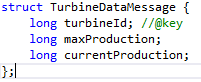
\includegraphics[width=0.3\textwidth,natwidth=250,natheight=200]{turbineDataMessage.PNG} 
	\captionsetup{format=plain,font=footnotesize,labelfont={bf,defaultCapFont},labelsep=quad,singlelinecheck=no}
	\caption[Centralized turbine reply message]{
		\label{fig:cenTurbineDataMessage} 
		\footnotesize{%
			The the reply message .idl file sent from the turbines to the Park Pilot in the centralized solution.
		}
	}
\end{figure}

The IDL definitions are are defined from looking at what data to transfer between the turbines and the Park Pilot. \Cref{fig:cenTurbineDataMessage} for example is IDL definition of the data transfer object used as reply from the turbines to the Park Pilot. 

%\subsection{Topics}
%
%Including the topics generated from the RTI Connext Request-Reply implementation~\cite{rtiConnextUsersManual} the following topics are used:
%
%\begin{figure}
%	\centering
%	\begin{tikzpicture}[
	point/.style={inner sep=0pt}, %circle,minimum size=2pt,fill=red},
	textNode/.style={inner sep=2pt},
	hv path/.style={to path={-| (\tikztotarget)}},
	vh path/.style={to path={|- (\tikztotarget)}},
	skip loop h/.style={to path={-- ++(0,#1) -| (\tikztotarget)}},
	skip loop v/.style={to path={-- ++(#1,0) |- (\tikztotarget)}},
	graphs/every graph/.style={edges=rounded corners}
	]
	
% Place nodes
\matrix[row sep=1.4cm,column sep=.4cm] {
	\node [point]  		(p1x1)	{}; &&
	\node [rectangle]	(Turbine)		[draw, label=above:\textbf{$\cdot$}N Turbines, text width=50pt]	{Cur.Prod. Max.Prod}; &&
	\node [point]  		(p1x3)	{}; \\
	
	\node [point]  		(p2x1)			{}; &&
	\node [textNode]	(HPPP)		 	{Reg. algorithm}; &&
	\node [textNode]	(Setpoint)	{N Setpoints}; \\

	&& \node [textNode]  (gSetpoint)							{Global SetPoint}; \\
};
	
\graph[use existing nodes]{
	Turbine ->[skip loop v=-3.1cm] HPPP -> Setpoint ->[vh path] Turbine;
	gSetpoint -> HPPP;
};

\end{tikzpicture}



%\begin{tikzpicture}[
%	point/.style={inner sep=0pt}, %circle,minimum size=2pt,fill=red},
%	textNode/.style={inner sep=2pt},
%	hv path/.style={to path={-| (\tikztotarget)}},
%	vh path/.style={to path={|- (\tikztotarget)}},
%	skip loop h/.style={to path={-- ++(0,#1) -| (\tikztotarget)}},
%	skip loop v/.style={to path={-- ++(#1,0) |- (\tikztotarget)}},
%	graphs/every graph/.style={edges=rounded corners}
%	]
%	
%% Place nodes
%\matrix[row sep=1.5cm,column sep=.5cm] {
%	\node [point]  		(p1x1)	{}; &&
%	\node [rectangle]	(Turbine)		[draw, label=above:\textbf{$\cdot$}N Turbines, text width=50pt]	{Cur.Prod. Max.Prod}; &&
%	\node [point]  		(p1x3)	{}; \\
%	
%	\node [point]  		(p2x1)			{}; &&
%	\node [textNode]	(HPPP)		 	{HPPP}; &&
%	\node [textNode]	(Setpoint)	{\textbf{$\cdot$}N Setpoints}; \\
%
%	\node [textNode]  (gSetpoint)										{Global SetPoint}; &&
%	\node [rectangle]	(Data)			[draw, text width=50pt] {Cur.prod  Max.Prod};\\
%};
%
%\node [textNode,right of=Data] {~~~~~~~~~~~~~~~~~\textbf{$\cdot$}N Turbines};
%	
%\graph[use existing nodes]{
%	Turbine ->[skip loop v=-2.7cm] HPPP -> Setpoint ->[vh path] Turbine;
%	gSetpoint.east -> HPPP;
%	Data -> HPPP;
%};
%
%\end{tikzpicture}
%
%	\captionsetup{format=plain,font=footnotesize,labelfont={bf,defaultCapFont},labelsep=quad,singlelinecheck=no}
%	\caption[Regulation aslgorithm input/output parameters]{
%		\label{fig:ioRegAlg} 
%		\footnotesize{%
%			Input/output parameters of the regulation algorithm.
%		}
%	}
%\end{figure}

\subsection{Choosing quality of service parameters}\label{sec:choosingQosParams}

Quality of service (QoS) parameters are parameters used to determine system behavior. As such, setting the right ones for our system is important in order to get the centralized solution to behave as much as the current system at Siemens as possible. 

In order to decide the QoS parameters for the centralized solution, the QoS XML file from the current system at Siemens was provided by Siemens (see \cref{appendix:siemensQosFile} for the QoS XML file). Thus QoS parameters for the centralized solution has been set using this file, which presents many different QoS profiles.

The Siemens QoS XML file only specifies one \textit{DomainParticipantFactory} profile. Thus, this factory profile has been applied to the solution and only parameters irrelevant to the purpose of this thesis has been removed from the profile. 

The Siemens QoS XML file specifies two \textit{DomainParticipant} profiles. One using UDPv4 and one using DTLS as transport plugin. The one using UDPv4 has been chosen for the centralized solution, since DTLS encryption and decryption is an unnecessary overhead, that either should be introduced to both the centralized- and the decentralized solution or to neither, for the two solutions to be compared on the same terms. Thus for simplicity reasons introducing DTLS to neither of the solutions has been chosen.

As for \textit{DataReaders}, \textit{DataWriters} and \textit{Topics}, the file specifies many different profiles and where each profile has been applied to the current system at Siemens has not been informed by Siemens. Thus we don't know which ones has been used for the part of the system that is implemented with the centralized solution. 

Each parameter in every QoS profile has been evaluated and the parameters relevant to the purpose of this theses has been applied to the centralized solution, based on assumptions about the current Siemens system. The QoS XML file roughly presents profiles that combines the following parameters in different ways:

\paragraph{Reliability} is the parameter, which determines whether or not data published by a DataWriter will be reliably delivered by the DDS framework to matching DataReaders~\cite{rtiConnextUsersManual}. The three levels of reliability presented by the different profiles are:

\begin{itemize}
	\item \textbf{Best effort reliability} profiles are configured so data samples are sent once and missed samples are acceptable.
	\item \textbf{Reliable} profiles are configured to make sure that data sent is received and missed samples are resent. DataWriters will send samples reliably to DataReaders, buffering sent data until they have been acknowledged as being received by DataReaders and resending any samples that may have been lost during transport. The DataWriter buffer of this configuration is set to the size of one message, which means only the newest message are resent. This implies that an unacknowledged sample may be overwritten and thus lost. 
	\item \textbf{Strictly reliable} profiles are configured exactly like reliable profiles, but with a larger DataWriter buffer. Increasing the DataWriter buffer size will decrease the chance of unacknowledged samples being overwritten. Thus DataReaders are ensured all messages sent by the DataWriters.
\end{itemize}

\paragraph{Durability} controls whether or not, and how, published samples are stored by the DataWriter application for DataReaders that are found after the samples were initially written, thus allowing new DataReaders to receive data sent before they were created. The levels of durability presented by the different profiles are:

\begin{itemize}
	\item \textbf{No durability} profiles are configured not to store any samples for newly discovered DataReaders.
	\item \textbf{Local durability} profiles are configured so that DataWriters will store and send previously published samples for delivery to newly discovered DataReaders as long as the DataWriter still exists.
\end{itemize}

\paragraph{Throughput} is configured using the batch~\cite{rtiConnextUsersManual} parameter, which can be used to decrease the amount of communication overhead associated with the transmission and (in case of reliable communication) acknowledgment of small samples at the expense of latency. This is done by batching many smaller samples to be sent in a single large packet, which increases network utilization and thus throughput in terms of samples per second. The two levels of throughput presented by the different profiles are:

\begin{itemize}
	\item \textbf{Regular throughout} profiles are configured not batch any samples, thus data samples and (in case of reliable communication) acknowledgment message are sent individually.
	\item \textbf{High throughput} profiles are configured so DataWriters will batch data in order to increase throughput.
\end{itemize}

The many profiles in the Siemens QoS XML file (\cref{appendix:siemensQosFile}) are presumably made for many different purposes. For building the centralized solution, the profile using \textbf{Strictly reliable}, \textbf{No durability} and \textbf{Regular throughput} configurations was chosen based on the following assumptions about the current Siemens system:

\begin{itemize}
	\item \textbf{Strictly reliable} messaging is important for the Park Pilot to compute setpoints for each turbine, since states of all turbines are needed in order to calculate setpoints. Thus resending a sample data if the sample data is dropped is needed in order to calculate setpoints. 
	\item \textbf{No durability} is needed for the regulation algorithm. If a new turbine is discovered, the turbine have no need of receiving old requests or setpoints. The turbine only needs to make itself available to requests from the Park Pilot and thereby be taken into account, which is done automatically by \textit{Connext} when a new DataReader is discovered.  
	\item \textbf{Regular throughput} provides the best performance for the regulation cycle. Batching data samples does not make any sense for the centralized solution since during the regulation cycle, a given node maximum can fall one message behind and since heartbeats and data samples are batched per default.
\end{itemize}

The profile from the current Siemens system QoS XML file chosen for the centralized solution is \textit{SwpStrictReliableNoDurability} (\cref{appendix:siemensQosFile}). All parameters of the quality of service configuration for the centralized solution is presented and evaluated in section \cref{sec:detailedQoSDesc}.


\subsection{Detailed quality of service evaluation} \label{sec:detailedQoSDesc}


The section provides a detailed evaluation of every parameter of the chosen profiles of the centralized solution QoS XML file, including the QoS parameters deemed irrelevant and thereby removed from the QoS file provided by Siemens (\cref{appendix:siemensQosFile}). See \cref{appendix:centralizedQosFile} for centralized solution QoS XML file. Removed parameters are marked with '(removed)' and commented out in the figures.

\paragraph{Participant factory} (\cref{fig:parFacQos}) QoS parameters has been evaluated as follows:

\begin{itemize}
	\item \textbf{autoenable\_created\_entities (removed)} determines whether or not participants should be enabled upon initialization. For the centralized solution the default value (enabled) for this parameter is sufficient.
	\item \textbf{logging} is set for all participants and occurs on both errors and warning messages concerning the underlying platform (hardware or OS) on which \textit{RTI Connext} is running, where a warning indicates that \textit{RTI Connext} is taking an action that may of may not be what was intended. This parameter is set since the current system uses this setting but also for debugging purposes.
\end{itemize}

\begin{figure}
\begin{lstlisting}[language=XML]
<participant_factory_qos>
	<!--entity_factory>
		<autoenable_created_entities>false</autoenable_created_entities>
	</entity_factory-->
	<logging>
		<verbosity>WARNING</verbosity>
		<category>PLATFORM</category>
		<print_format>VERBOSE_TIMESTAMPED</print_format>
		<output_file>ddsadaptor.log</output_file>
	</logging>
</participant_factory_qos>
\end{lstlisting}
\caption[Participant factory QoS parameters]{
		\label{fig:parFacQos} 
		\footnotesize{Participant factory QoS parameters.}
	}
\end{figure}

\paragraph{Participant} (\cref{fig:parQos}) QoS parameters has been evaluated as follows:
 
\begin{itemize}
	\item \textbf{database} configures how \textit{RTI Connext} manages its internal database, which stores information about entities created locally as well as remote entities found during the discovery process. Database thread has been set to wake up and delete removed records 1 ns after a given domain participant is destroyed for cleanup purposes. 
	\item \textbf{transport\_builtin} configures the built-in transport plugins (UDPv4/IP, UDPv6/IP, TCP/IP, TLS, DTLS, shared memory, etc.) used by the \textit{DomainParticipants}. By default UDPv4 and shared memory plugins are enabled. For the centralized solution, the shared memory plugin is disabled (set to UDPv4 only) so that applications running on the same node don't use shared memory to communicate. This is done since our test setup only involves 3 PC's, each simulating many turbines. As such, communication through shared memory is not acceptable.
	\item \textbf{receiver\_pool (removed)} configures the internal \textit{Connext} thread used to process the data received from a transport. As such, the \textbf{buffer\_size} configures the size of the receive buffer in bytes. The default value of this property set to the largest message size of all installed transports, which is needed for the centralized solution and thus removed from the centralized solution QoS file.
	\item \textbf{ignore\_nonup\_interfaces (removed)} property allows/disallows the use of interfaces that are not reported as UP (by the operating system) in the UDPv4 transport. Setting this value to 0 supports the communication scenarios in which interfaces are enabled after the participant is created. This parameter has been removed since the centralized solution do not have any interfaces that are enabled after the participant is created. Thus the centralized solution uses the default value of 1 which means interfaces that are reported as down is not supported.
	\item \textbf{multicast\_enabled (removed)} parameter is used to configure if the transport plugin (in this case UDPv4) should use multicast for sending and receiving. By removing this parameter the default value is used, which allows multicast on all network interfaces allowed for multicast that is found up and running when the plugin is instantiated. The centralized solution is \textbf{not} supposed to use multicast for sending and receiving data used in context of the regulation algorithm, however multicast is acceptable for discovery of \textit{DomainParticipants}. Thus this parameter is set to default for discovery purposes.
	
	Note that we have not set any multicast addresses on the \textit{DataReader} QoS profile (see DataReader QoS parameters later in this section), which means multicast is not used for sending and receiving data in the context of the regulation algorithm.  
	\item \textbf{message\_size\_max} configures the maximum size of a message in bytes. This value must be set before the transport plugin is registered, so that \textit{Connext} can properly use the plugin. For the purpose of the centralized solution this value is more or less irrelevant, since it's only a max value. The value of this parameter just have to be larger than the largest message plus any overhead (ie. $message\_size\_max >= largest\_msg + msg\_overhead$). The largest message of the centralized solution contains $3\cdot64bit=192bit$. Thus to be mimic the current Siemens system and since any larger value has no influence on our test results, the value of this parameter is left as the same value used by the current system at Siemens of 65535 bytes.
	\item \textbf{send\_socket\_buffer\_size} configures the size of the send buffer in bytes. This value must be greater than or equal to the value of the \textit{message\_size\_max} parameter. For the purpose of the centralized solution this value have to be big enough to contain enough messages to cover \textit{DataWriter} history QoS (see DataWriter QoS history parameter later in this section), with regards to the largest centralized message size of $3\cdot64bit=192bits$ plus any message overhead. Thus a value of 65535 bytes is more than enough, and the value is kept to mimic the current Siemens system and since any larger value has no influence on our test results.
	\item \textbf{recv\_socket\_buffer\_size} configures the size of the receive buffer. This value must be greater than or equal to the value of the \textit{message\_size\_max} parameter. For the purpose of the centralized solution this value just have to be big enough to contain enough messages to cover \textit{DataReader} history QoS (see DataReader QoS history parameter later in this section) with regards to the largest centralized message size of $3\cdot64bit=192bits$ plus any message overhead. 
\end{itemize}

\begin{figure}
\begin{lstlisting}[language=XML]
<participant_qos>
	<database>
		<shutdown_cleanup_period>
			<sec>DURATION_ZERO_SEC</sec>
			<nanosec>1</nanosec>
		</shutdown_cleanup_period>
	</database>
	<participant_name>
		<name>Siemens Wind Power DDS Adaptor</name>
	</participant_name>
	<transport_builtin>
		<mask>UDPv4</mask>
	</transport_builtin>
	<!--receiver_pool>
		<buffer_size>65535</buffer_size>
	</receiver_pool-->
	<property>
		<value>
			<!--element>
				<name>dds.transport.UDPv4.builtin.ignore_nonup_interfaces</name>
				<value>0</value>
			</element>
			<element>
				<name>dds.transport.UDPv4.builtin.multicast_enabled</name>
				<value>0</value>
			</element-->
			<element>
				<name>dds.transport.UDPv4.builtin.parent.message_size_max</name>
				<value>65535</value>
			</element>
			<element>
				<name>dds.transport.UDPv4.builtin.send_socket_buffer_size</name>
				<value>65535</value>
			</element>
			<element>
				<name>dds.transport.UDPv4.builtin.recv_socket_buffer_size</name>
				<value>2097152</value>
			</element>
		</value>
	</property>
</participant_qos>
\end{lstlisting}
\caption[Participant QoS parameters]{
		\label{fig:parQos} 
		\footnotesize{Participant QoS parameters.}
	}
\end{figure}

\paragraph{Topic} QoS parameters are not presented by the Current Siemens System QoS XML file and thus no \textit{Topic} QoS profile has been applied to the centralized solution. 

\paragraph{DataWriter} QoS parameters has been set after the profile \textit{SwpStrictReliableNoDurability} from the current Siemens system QoS XML file (\cref{appendix:siemensQosFile}), as discussed in \cref{sec:choosingQosParams}. Combining the \textit{SwpStrictReliableNoDurability} profile with the two underlying base profiles (\textit{SwpReliableNoDurability} and \textit{SwpBestEffort}) we get the QoS parameters presented on \cref{fig:writerQoS}. The DataWriter parameters presented on \cref{fig:writerQoS} has been evaluated as follows:

\begin{itemize}
	\item \textbf{liveliness (removed)} configures how \textit{Connext} determines whether a \textit{DataWriter} is 'alive'. The \textit{lease\_duration} then specifies the maximum period at which packets that indicate that the \textit{DataWriter} is still alive are sent to matching \textit{DataReaders}. If this period is not met, an event is triggered on subscribers within the Topic, where the period wasn't reached. The centralized solution is not built to be fault tolerant or to detect any changes is number of turbines. Thus this parameter has been removed.
	\item \textbf{reliability} determines whether or not data published by a \textit{DataWriter} will be reliably delivered by \textit{Connext} to matching \textit{DataReaders}. As discussed in \cref{sec:choosingQosParams}, the centralized solution is built under the assumption that strictly reliable messaging is needed. Thus the reliability is configured for strictly reliable messaging with a max blocking time of the send queue of 5 seconds, as the current Siemens system.
	
	Note that strict reliability is only achieved when combining this parameter configuration with a \textit{KEEP\_ALL\_HISTORY\_QOS} history configuration.
	\item \textbf{history} configures the number of data samples that \textit{Connext} will store locally for \textit{DataWriters} and \textit{DataReaders}, applies on a per \textit{Topic} keyed instance basis. This parameter has been set to \textit{KEEP\_ALL\_HISTORY\_QOS} for strictly reliable messaging, which means \textit{Connext} will only store up to the value of the \textit{max\_samples\_per\-\_instance} of the \textit{resource\_limits} QoS parameter.
	\item \textbf{resource\_limits} determines how \textit{DomainParticipants} allocate and use physical memory for internal resources. In this case it's used to configure the maximum number of data samples of any one instance that \textit{Connext} will store for a \textit{DataWriter}. The centralized solution stores 20 unacknowledged data samples in the send queue, so data samples can be resent if a timeout occurs or a NACK message from a \textit{DataReader} is received. So the centralized solution is strictly reliable up to 20 unacknowledged messages pr. keyed instance, as the current Siemens System. Any more result in data samples being overridden by the \textit{DataWriter}.
	
	The value of 20 is kept for the centralized solution. Theoretically, for the purpose of the centralized solution, this value could be set to 1, since the centralized solution waits for responds and thus every \textit{DomainParticipant} is at most 1 message behind at any given time. However, since the centralized solution is set to run with strictly reliable messaging, this queue has to be set larger to prevent the turbines from blocking the regulation cycle, when waiting for ACK/NACK messages from the Park Pilot after sending a reply. Thus this value is set to be large enough to not impact the regulation cycle time, in which case 20 is fine. 
	\item \textbf{protocol} parameter provides the system developer control over the configurable portions of the standard protocol for packet exchange between applications, in this case the configuration of the reliable data delivery mechanism (\textit{rtps\_reliable\_writer}) of the protocol on a per \textit{DataWriter} basis. 
	
	The parameters within the \textit{protocol} parameter is used to tune the behavior of the reliability protocol. Setting them is not required in order to achieve strict reliability but is beneficial from a performance standpoint. Thus since this performance optimization is applied to the current Siemens system, we apply it to the centralized solution.
	
	The optimization consists of increasing and decreasing the rate at which heartbeats are sent to \textit{DataReaders} according to the samples within the \textit{DataWriter} send cache (set by the \textit{resource\_limit} parameter). If the cache is below 5 data samples, the rate at which heartbeats are sent is slowed down, indicating \textit{DataReaders} are getting data samples correctly, to reduce network traffic. Similarly, if the cache gets higher than 15 data samples, the heartbeat rate is increased to spur faster acknowledgment (positive or negative) of its samples to allow it to empty its cache and avoid blocking. The number of times the \textit{DataWriter} will a heartbeat to a reader without receiving a response is set to 500. After 500 sent heartbeats, the \textit{DataReader} will be considers inactive and the \textit{DataWriter} will no longer await acknowledgements before discarding sent data. This parameter is set to prevent a poorly behaving process from monopolizing the CPU for several seconds.
	
	Furthermore the \textit{DataWriters} of the centralized solution is set to be reactive, by setting the NACK response delay to 0 seconds. Leaving the centralized solution less reactive, one could increase the changes that the writer will learn of additional reader that missed the same data, in which case \textit{DataWriters} would be able to send a single multicast repair, instead of many unicast repairs, thereby using the available network bandwidth more efficiently. However since multicast is disabled, we set data to be resent immediately after receiving a NACK from a \textit{DataReader}. 
	
	Finally the \textit{min\_send\_window\_size} and \textit{max\_send\_window\_size} configures how many data samples are kept by in their send queue until acknowledgments from all of their subscribing \textit{DataReaders} has been received. These parameters has been removed since their values are overwritten by the \textit{resource\_limits} parameter having a lower value.
\end{itemize}

\begin{figure}
\begin{lstlisting}[language=XML]
<datawriter_qos>
	<!--liveliness>
		<lease_duration>
			<sec>1</sec>
			<nanosec>0</nanosec>
			</lease_duration>
	</liveliness-->
	<reliability>
		<kind>DDS_RELIABLE_RELIABILITY_QOS</kind>
		<max_blocking_time>
			<sec>5</sec>
			<nanosec>0</nanosec>
		</max_blocking_time>
	</reliability>
	<history>
		<kind>KEEP_ALL_HISTORY_QOS</kind>
	</history>
	<resource_limits>
		<max_samples_per_instance>20</max_samples_per_instance>
	</resource_limits>
	<protocol>
		<rtps_reliable_writer>
			<low_watermark>5</low_watermark>
			<high_watermark>15</high_watermark>
			<heartbeat_period>
				<sec>0</sec>
				<nanosec>100000000</nanosec>
			</heartbeat_period>
			<fast_heartbeat_period>
				<sec>0</sec>
				<nanosec>10000000</nanosec>
			</fast_heartbeat_period>
			<late_joiner_heartbeat_period>
				<sec>0</sec>
				<nanosec>10000000</nanosec>
			</late_joiner_heartbeat_period>
			<max_heartbeat_retries>500</max_heartbeat_retries>
			<min_nack_response_delay>
				<sec>0</sec>
				<nanosec>0</nanosec>
			</min_nack_response_delay>
			<max_nack_response_delay>
				<sec>0</sec>
				<nanosec>0</nanosec>
			</max_nack_response_delay>
			<!--min_send_window_size>32</min_send_window_size>
			<max_send_window_size>32</max_send_window_size-->
		</rtps_reliable_writer>
	</protocol>
</datawriter_qos>
\end{lstlisting}
\caption[DataWriter QoS parameters]{
		\label{fig:writerQoS} 
		\footnotesize{DataWriter QoS parameters.}
	}
\end{figure}

\paragraph{DataReader} QoS parameters has been set after the profile \textit{SwpStrictReliableNoDurability} from the current Siemens system QoS XML file (\cref{appendix:siemensQosFile}), as discussed in \cref{sec:choosingQosParams}. This is the same profile used to configure \textit{DataWriter} QoS. Combining the \textit{SwpStrictReliableNoDurability} profile with the two underlying base profiles (\textit{SwpReliableNoDurability} and \textit{SwpBestEffort}) we get the QoS parameters presented on \cref{fig:readerQoS}. The \textit{DataReaders} parameters presented on \cref{fig:readerQoS} has been evaluated as follows:

\begin{itemize}
	\item \textbf{liveliness (removed)} see \textit{DataWriter liveliness} QoS evaluation above for parameter description. 
	
	The centralized solution is not built to be fault tolerant or to detect any changes is number of turbines. Thus this parameter has been removed.
	
	\item \textbf{reliability} see \textit{DataWriter reliability} QoS evaluation above for parameter description.
	
	The centralized solution is configured for strictly reliable messaging.
	
	Note that strict reliability is only achieved when combining this parameter configuration with a \textit{KEEP\_ALL\_HISTORY\_QOS} history configuration.
	\item \textbf{history} see \textit{DataWriter history} QoS evaluation above for parameter description.
	
	Strict reliability is maintained through the \textit{KEEP\_ALL\_HISTORY\_QOS}, where \textit{resource\_limits} defines how many data samples the receive queue can hold.
	
	\item \textbf{resource\_limits} see \textit{DataWriter resource\_limits} QoS evaluation above for parameter description.
	
	The receive queue size of the \textit{DataReaders} are configured to 20 data samples per keyed instance. 
	\item \textbf{protocol} parameter provides the system developer control over the configurable portions of the standard protocol for packet exchange between applications, in this case the configuration of the reliable data reader mechanism (rtps\_reliable\_reader) of the protocol on a per \textit{DataReader} basis.
	
	The parameters within the \textit{protocol} parameter is used to tune the reliability protocol. Setting them is not required in order to achieve strict reliability but is beneficial from a performance standpoint. 
	
	When a \textit{DataReader} receives a heartbeat from a \textit{DataWriter} (indicating (a) that the DataWriter still exists on the network and (b) what sequence numbers it has published), the \textit{DataReader} will instantly reply with a positive or negative acknowledgment. Setting the \textit{response\_delay} to 0 nanoseconds makes the system more reactive at the cost of an increased chance of (N)ACK spikes. The regulation cycle blocks until messages from all turbines has been received, thus it is crucial to inform any data sample losses as soon as possible.
\end{itemize}


\begin{figure}
\begin{lstlisting}[language=XML]
<datareader_qos>
	<!-- <liveliness>
		<lease_duration>
			<sec>1</sec>
			<nanosec>0</nanosec>
		</lease_duration>
	</liveliness> -->
	<history>
		<kind>KEEP_ALL_HISTORY_QOS</kind>
	</history>
	<reliability>
		<kind>RELIABLE_RELIABILITY_QOS</kind>
	</reliability>
	<resource_limits>
		<max_samples_per_instance>20</max_samples_per_instance>
	</resource_limits>
	<protocol>
		<rtps_reliable_reader>
			<min_heartbeat_response_delay>
				<sec>0</sec>
				<nanosec>0</nanosec>
			</min_heartbeat_response_delay>
			<max_heartbeat_response_delay>
				<sec>0</sec>
				<nanosec>0</nanosec>
			</max_heartbeat_response_delay>
		</rtps_reliable_reader>
	</protocol>
</datareader_qos>
\end{lstlisting}
\caption[DataReader QoS parameters]{
		\label{fig:readerQoS} 
		\footnotesize{DataReader QoS parameters.}
	}
\end{figure}


\section{Comparison to the current system at Siemens Wind Power}
The centralized solution presented in this chapter is based on the available information about the current Siemens systems, assumptions added about the parts that are unknown and a limited number of features implemented in the decentralized solution. In order to describe the difference, presented as a delta in \cref{fig:projectDiffOverviewCentralizedSiemens}, between the centralized solution and current Siemens system this must be taken into account.

\begin{figure}[!h]
	\centering
	\begin{tikzpicture}[
	node distance = 0.3cm,
	auto,
	block/.style={draw, rectangle, text width=5em, text centered, minimum height=5cm}		
	]
% Place nodes
\node [block]			(Siemens)												[label=above:Siemens system]	{};
\node []					(SimCen)		[right = of Siemens] 	{$\Delta$};
\node [block]			(OurCent)		[right = of SimCen] 	[label=above:Centralized solution]	{};

\end{tikzpicture}
	\captionsetup{format=plain,font=footnotesize,labelfont={bf,defaultCapFont},labelsep=quad,singlelinecheck=no}
	\caption[Comparison of the current Siemens system and the centralized solution]{
		\label{fig:projectDiffOverviewCentralizedSiemens} 
		\footnotesize{%
			Comparison of the current Siemens system and the centralized solution.
		}
	}
\end{figure}

Available information:

\begin{enumerate}
	\item Quality of Service profile from the current Siemens system.
	\item General overview of the regulation algorithm.
	\item Wind data generated by turbines in a Siemens Wind Power wind farm.
\end{enumerate}

The QoS profile created for the centralized solution is based on the QoS profile delivered by Siemens Wind Power. The difference between the two QoS profiles is that QoS parameters that have no influence on the results of the experiments performed has been removed from the QoS profile used by the centralized solution.
Based on the general overview of the regulation cycle used in the current Siemens system a naive regulation cycle has been created for the centralized solution. This cycle consists of the same steps as the ones in the current Siemens system thus the communication between the Park Pilot and the turbines is the same as the ones in the current Siemens solution in terms of packets sent and time spent waiting for reply. Since the centralized approach to communication in the current Siemens solution is one of the key reasons for the scalability problems of the system it is very important to duplicate this in the centralized solution.
The wind data generated by turbines in one of Siemens Wind Powers wind farms is used to regulate the max production of the turbines such that the regulation cycle is run on data from a realistic scenario.

Assumptions about the current Siemens system:

\begin{enumerate}
	\item \label{assumption1} The Park pilot must wait for replies from all turbines in order to correctly calculate setpoints.
	\item \label{assumption2} Messages must be reliably sent and received between the turbines and the Park Pilot.
	\item \label{assumption3} Calculation of an individual setpoint is done by dividing the global setpoint with the number of turbines.
	\item \label{assumption4} The amount of data needed in order to perform wind farm regulation is the global setpoint, number of turbines, maximum power production of the individual turbine and current power production of the individual turbine.  
\end{enumerate}

Assumption \ref{assumption1} and \ref{assumption2} is linked together. If the Park Pilot must wait for replies from all turbines in order to calculate setpoints, messages between turbines and the Park Pilot must be reliably delivered or else the system may end up in deadlock. Assumption \ref{assumption3} and \ref{assumption4} relates to the regulation algorithm.
Since the regulation algorithm used in the current Siemens system is unknown a naive regulation algorithm is used in the centralized solution. As a consequence the data needed for the regulation algorithm is limited. The global setpoint divided between the turbines gives the individual setpoints. If a turbine is unable to produce power enough to reach the individual setpoint the remaining power production is split between the turbines that are able to produce more power.

Features omitted from the centralized solution:

\begin{enumerate}
	\item \label{limitation1} Cluster implementation of current Siemens system.
	\item \label{limitation2} Recovery of turbines if they loose network connection.
	\item \label{limitation3}Data aggregation, data storage, external communication, noise control, flicker control, Ice control etc.
\end{enumerate}

The current Siemens system provides a number of features which are not implemented in the centralized solution. Most notably the current Siemens system is implemented with several Park Pilots making a wind farm into a collection of clusters. The centralized solution only has one Park Pilot. The problem of scalability in the current Siemens system is grounded in the lack of scalability when increasing the number of turbines for a single Park Pilot. Thus using only one Park Pilot in the centralized solution is enough to show the scalability problem of the current Siemens system, and create a basis for comparison to a decentralized model.
Another feature that is not implemented in the centralized solution is the ability for a turbine to recover from the loss of network. This feature is omitted because it has no real influence on the scalability of the centralized solution.
The features listed in omitted features \ref{limitation3} is all features of the Wind Power Supervisor. Since this thesis focus on the scalability and feasibility of a decentralized implementation of the Park Pilot the Wind Power Supervisor and its features has not been duplicated.

In summary the delta between the current Siemens system and the centralized solution consist of assumptions about the unknown parts of the current Siemens system and omitted features that has no influence on scalability.

%The delta between the current Siemens system and the centralized solution must be minimized in order to ensure that the centralized solution is as similar to the current Siemens system as possible. This will enable the results of a comparison between the centralized solution and the decentralized solution to be as close as possible to a comparison between the current Siemens solution and the decentralized solution.